\documentclass{article}
\usepackage[utf8]{inputenc}
\usepackage[margin = 0.8in]{geometry}
\usepackage{graphicx}
\usepackage{amsmath, amssymb}
\usepackage{subcaption}
\usepackage{multirow}
\usepackage{mathtools}
\usepackage{float}


\title{RBE595 - Week 5 Assignment}
\author{Keith Chester}
\date{Due date: February 12, 2023}

\begin{document}
\maketitle

\section*{Problem 1}
\textit{When is it suited to apply Monte-Carlo to a problem?}

Monte-Carlo is best applied to problems where the state is not well known and not easy/possible to simulate, and/or the environment has stochastic outcomes. Likewise, Monte-Carlo excels in episodic situations where either many episodes can be ran through or simulated in order to train. Monte-Carlo methods provide an estimation of a reward given a pair of (state, action), usually via an average of returns for the resulting action of that state. In this way Monte-Carlo will eventually converge to the true value of an optimal policy.


\section*{Problem 2}
\textit{When does the Monte-carlo prediction performs the first update? }

In Monte-Carlo prediction, the model performs its first update after the very first episode is completed. The returns are averaged for ecah (state, action) pair visited throughout the episode.

\section*{Problem 3}
\textit{What is off-policy learning and why it is useful? }


Off-policy learning is an approach in reinforcement learning where the policy utilized to explore and generate data (behavior policy) is different from the policy utilized for evaluation (target policy), unlike on-policy learning. This approach is useful, as it empowers the agent to learn a broader range of experiences.

Expanding on this, the on-policy can be described as soft, meaning that $\pi(a|s)>0$ for all $s\epsilon S$ and all $a \epsilon A(S)$, gradually moving close to the optimal policy. If we hope to continue exploration to continue to find a more optimal policy, we have to use a less optimal policy (like $\epsilon$-greedy) such that we sometimes perform unoptimally. Off-policy learning has the behavior policy explore for us, so the target policy can act optimally. This can lead to more stable behavior from the target policy that an on-policy approach could experience.

\section*{Problem 4}
\textit{Consider an MDP with a single nonterminal state and a single action that transitions back to the nonterminal state with probability $p$ and transitions to the terminal state with probability $1-p$. Let the reward be $+1$ on all transitions, and let $\gamma=1$. Suppose you observe one episode that lasts $10$ steps, with a return of $10$. What are the first-visit and every-visit estimators of the value of the nonterminal state? }

In this problem, first we consider the first-look estimator as it's the simplest. Here, $V=10$ as that is the outcome of the episode.

For the every-visit estimator, we must consider the reward we've accumulated at each step and average them. Thus, the every-visit estimator is calculated as:

\begin{equation}
    V= \frac{10+9+8+7+6+5+4+3+2+1}{10} = \frac{55}{10} = 5.5
\end{equation}

\section*{Problem 5}
\textit{In learning curves such as those shown in Figure 5.3 error generally decreases with training, as indeed happened for the ordinary importance-sampling method. But for the weighted importance-sampling method error first increased and then decreased. Why do you think this happened?}

\begin{figure}
    \centering
    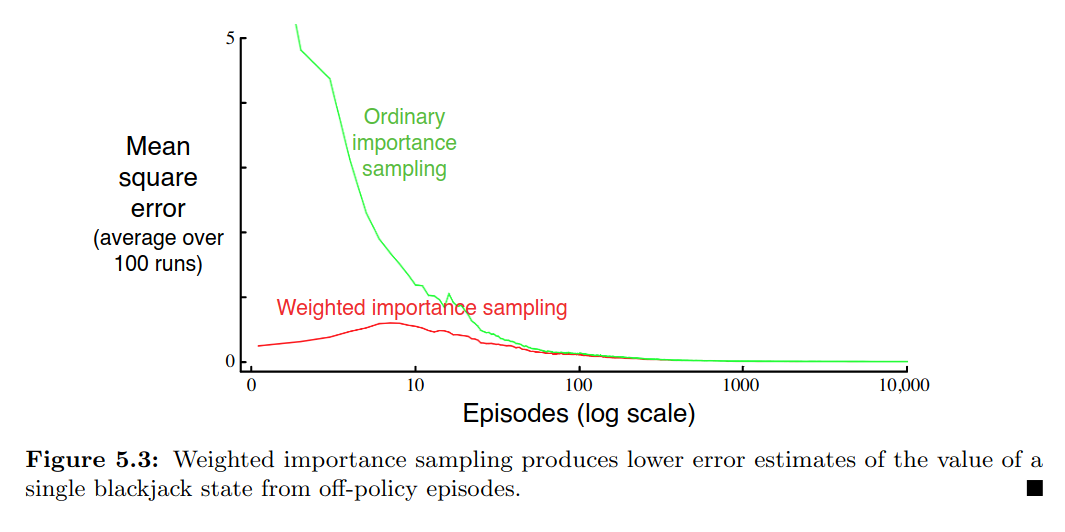
\includegraphics[width = 0.8\textwidth]{imgs/figure53.png}
    \caption{figure 5.3 from the book}
    \label{fig:problem5}
\end{figure}

Weighted importance sampling has an initial bias that results in an increase in error at the beginning, but then ultimately fades away through training.

\section*{Problem 6}
\textit{The results with Example 5.5 and shown in Figure 5.4 used a first-visit MC method. Suppose that instead an every-visit MC method was used on the same problem. Would the variance of the estimator still be infinite? Why or why not?}

\begin{figure}
    \centering
    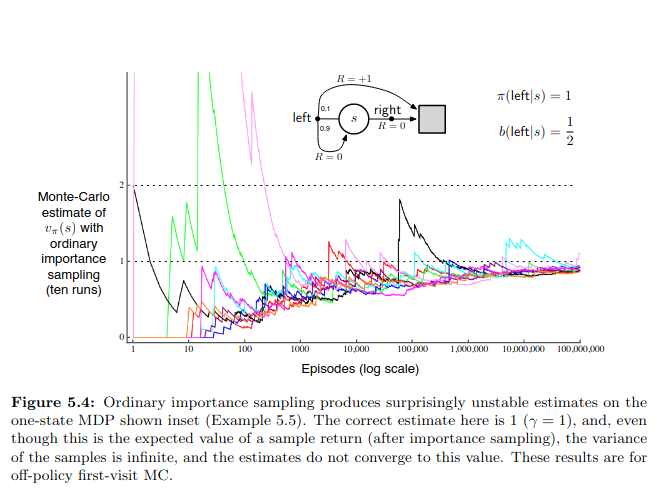
\includegraphics[width = 0.8\textwidth]{imgs/figure54.png}
    \caption{figure 5.4 from the book}
    \label{fig:problem6}
\end{figure}

In this example, we can represent each vist through the equation:

\begin{equation}
    E_b \bigg[
        \prod_{t=0}^{T-1} \bigg(\frac{\pi_t(A_t | S_t)}{\pi_b(A_t | S_t)} G_0 \bigg)^2
        \bigg]
\end{equation}

...where $\pi_t$ is our target policy and $\pi_b$ is our behavior policy. Future visits would utilize the equation:

\begin{equation}
    E_b \bigg[
        \frac{1}{T-1}
        \sum_{k=1}^{T-1}
        \prod_{t=0}^{T-1} \bigg(\frac{\pi_t(A_t | S_t)}{\pi_b(A_t | S_t)} G_0 \bigg)^2
        \bigg]
\end{equation}

Thus we can begin calculating each episode:

...our first episode is:

\begin{equation}
    E_{b_0} = \frac{1}{2}(0.1)(\frac{1}{0.5})^2
\end{equation}

...our second episode contains our first visit:

\begin{equation}
    E_{b_1} = \frac{1}{2} \bigg( \frac{1}{2} (0.9) \frac{1}{2} (0.1) (\frac{1}{0.5}\frac{1}{0.5})^2 + E_{b_0} \bigg)
\end{equation}

...where our second visit is represented as that part multiplied by the fraction (or $2*E_{b_1}$)...

...and our third equation contains the first two:

\begin{equation}
    E_{b_2} = \frac{1}{3} \bigg( \frac{1}{2} (0.9)\frac{1}{2} (0.9) \frac{1}{2} (0.1) (\frac{1}{0.5}\frac{1}{0.5}\frac{1}{0.5})^2 + 2*E_{b_1} \bigg)
\end{equation}

...and so on. We can represent this as

\begin{equation}
    0.1 \sum_{k=1}^{\infty}\frac{1}{k} \sum_{i=0}^{k-1} (0.9)^i 2^i 2
\end{equation}

...which we can simplify by bringing the $2$ to the front and combining our $n^i$ values:

\begin{equation}
    0.2 \sum_{k=1}^{\infty}\frac{1}{k} \sum_{i=0}^{k-1} (1.8)^i
\end{equation}

Since we ee that we that we are taking the sum an infinite amount of times, we can safely say that this is infinite variance.

\section*{Problem 7}

\textit{Derive the weighted-average update rule (5.8) from (5.7). Follow the pattern of the derivation of the unweighted rule (2.3).}

We start with, from 5.7, the equation for $V_n$:

\begin{equation}
    V_n \dot{=} \frac{\sum_{k=1}^{n-1}W_k G_k}{\sum_{k=1}^{n-1} W_k}, n \geq 2
\end{equation}

...and also reference 5.8, our update rule, which is our target:

\begin{equation}
    V_{n+1} \dot{=} V_n + \frac{W_n}{C_n}\bigg( G_n-V_n \bigg), n\geq 1
\end{equation}

also, we know that

\begin{equation}
    C_{n+1} \dot{=} C_n + W_{n+1}\dots
\end{equation}

...where $C_0 \dot{=} 0$ and $V_1$ is arbitray and doesn't need to be specified, where $C$ represents the sum of our weights.

We can then express start wth $V_{n+1}$, and derive:

\begin{equation}
    V_{n+1} \dot{=} \frac{\sum_{k=1}^{n}W_k G_k}{\sum_{k=1}^{n} W_k}
\end{equation}

\begin{equation}
    V_{n+1} = \frac{W_n G_n + \sum_{k=1}^{n-1}W_k G_k}{\sum_{k=1}^{n-1} W_k} \frac{\sum_{k=1}^{n-1}W_k}{\sum_{k=1}^{n-1} W_k}
\end{equation}

...the right-most component cancels at this point to 1, leaving us with:

\begin{equation}
    V_{n+1} = \frac{W_n G_n + \sum_{k=1}^{n-1}W_k G_k}{\sum_{k=1}^{n-1} W_k}
\end{equation}

...then we can introduce $C_n$ as, again, it is the sum of our weights:

\begin{equation}
    V_{n+1} = \bigg(\frac{W_n G_n}{C_{n-1}} + V_n \bigg) \frac{C_{n-1}}{C_n}
\end{equation}

\begin{equation}
    V_{n+1} = \frac{W_n G_n + V_n C_{n-1}}{C_n}
\end{equation}

We can use a trick to add $V_n$ to the equation below by also removing it, so our equation is still equivalent.

\begin{equation}
    V_{n+1} = \frac{W_n G_n + V_n C_{n-1}}{C_n} + V_n - V_n
\end{equation}

We rearrange to keep $V_n$ up front and integrate the $-V_n$ to our fraction. We're going to break apart the fraction as well to keep things easier.

\begin{equation}
    V_{n+1} = V_n + \frac{W_n G_n}{C_n} + \frac{V_n C_{n-1}- V_n C_n}{C_n}
\end{equation}

\begin{equation}
    V_{n+1} = V_n + \frac{W_n G_n}{C_n} - \frac{V_n W_n} {C_n}
\end{equation}

...finally we can pull out $\frac{W_n}{C_n}$ as like terms:

\begin{equation}
    V_{n+1} = V_n + \frac{W_n}{C_n} \bigg(G_n - V_n \bigg)
\end{equation}

...which is what we set out to prove!

\section*{Problem 8}
\textit{In the boxed algorithm for off-policy MC control, you may have been expecting the $W$ update to have involved the importance-sampling ratio $\frac{\pi(A_t|S_t)}{b(A_t|S_t)}$, but instead it involves $\frac{1}{b(A_t|S_t)}$. Why is this nevertheless correct?}

Since $\pi$ is a deterministic policy, the probability of it being taken is always 1. Thus $\frac{1}{b(A_t|S_t)}$ is still correct.


\end{document}